
%(BEGIN_QUESTION)
% Copyright 2010, Tony R. Kuphaldt, released under the Creative Commons Attribution License (v 1.0)
% This means you may do almost anything with this work of mine, so long as you give me proper credit

Anta at et voltmeter viser 22 volt mellom testpunktene {\bf A} og {\bf D}:

$$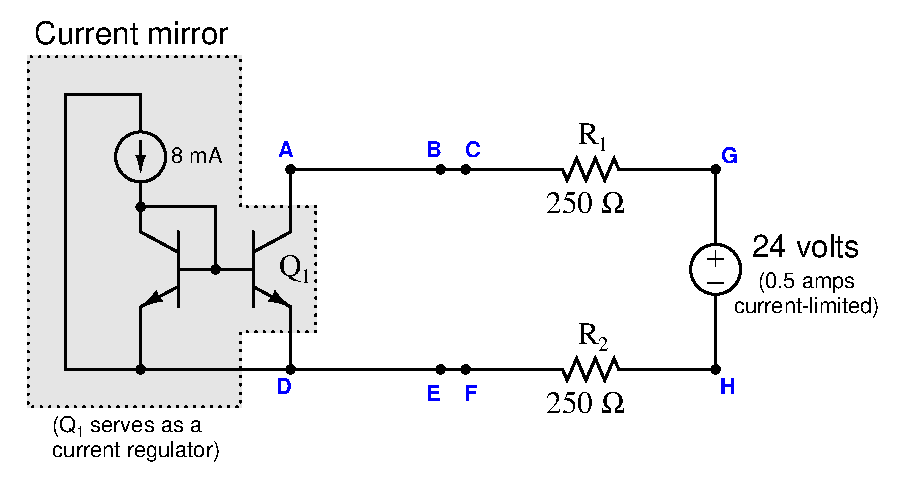
\includegraphics[width=15.5cm]{i00773x01.eps}$$

Vurder sannsynligheten for hver oppgitt feil i denne kretsen. Vurder én feil om gangen (dvs. ingen sammenfallende feil), og avgjør om hver feil alene kan forklare {\it alle} målinger og symptomer i kretsen.

% No blank lines allowed between lines of an \halign structure!
% I use comments (%) instead, so that TeX doesn't choke.

$$\vbox{\offinterlineskip
\halign{\strut
\vrule \quad\hfil # \ \hfil &
\vrule \quad\hfil # \ \hfil &
\vrule \quad\hfil # \ \hfil \vrule \cr
\noalign{\hrule}
%
% First row
{\bf Feil} & {\bf Mulig} & {\bf Umulig} \cr
%
\noalign{\hrule}
%
% Another row
$R_1$ feilet åpen &  &  \cr
%
\noalign{\hrule}
%
% Another row
$R_2$ feilet åpen &  &  \cr
%
\noalign{\hrule}
%
% Another row
$Q_1$ feilet åpen &  &  \cr
%
\noalign{\hrule}
%
% Another row
$R_1$ feilet kortsluttet &  &  \cr
%
\noalign{\hrule}
%
% Another row
$R_2$ feilet kortsluttet &  &  \cr
%
\noalign{\hrule}
%
% Another row
$Q_1$ feilet kortsluttet &  &  \cr
%
\noalign{\hrule}
%
% Another row
Spenningskilde død &  &  \cr
%
\noalign{\hrule}
} % End of \halign
}$$ % End of \vbox

Til slutt: angi {\it neste} diagnostiske test eller måling du ville gjort på dette systemet. Forklar hvordan resultatet/resultatene av denne testen bidrar til å avklare plassering og/eller type feil.

\vfil

\underbar{file i00773}
\eject
%(END_QUESTION)





%(BEGIN_ANSWER)

% No blank lines allowed between lines of an \halign structure!
% I use comments (%) instead, so that TeX doesn't choke.

$$\vbox{\offinterlineskip
\halign{\strut
\vrule \quad\hfil # \ \hfil &
\vrule \quad\hfil # \ \hfil &
\vrule \quad\hfil # \ \hfil \vrule \cr
\noalign{\hrule}
%
% First row
{\bf Feil} & {\bf Mulig} & {\bf Umulig} \cr
%
\noalign{\hrule}
%
% Another row
$R_1$ feilet åpen &  & $\surd$ \cr
%
\noalign{\hrule}
%
% Another row
$R_2$ feilet åpen &  & $\surd$ \cr
%
\noalign{\hrule}
%
% Another row
$Q_1$ feilet åpen &  & $\surd$ \cr
%
\noalign{\hrule}
%
% Another row
$R_1$ feilet kortsluttet & $\surd$ &  \cr
%
\noalign{\hrule}
%
% Another row
$R_2$ feilet kortsluttet & $\surd$ &  \cr
%
\noalign{\hrule}
%
% Another row
$Q_1$ feilet kortsluttet &  & $\surd$ \cr
%
\noalign{\hrule}
%
% Another row
Spenningskilde død &  & $\surd$ \cr
%
\noalign{\hrule}
} % End of \halign
}$$ % End of \vbox


%(END_ANSWER)





%(BEGIN_NOTES)


%INDEX% Feilsøkingsrepetisjon: elektriske kretser

%(END_NOTES)


